\chapter{Policy Optimisation}
\label{chap:3_Optimisation}

\section{Overview}

With the theoretical base of reinforcement learning established, we will look into the idea of policy gradients methods, and how it is used in Actor-Critic methods. Finally, the main characteristics of the DDPG and PPO algorithms will be reviewed.

As briefly mentioned in section \ref{sec:2_6_modelFreeContinuous}, the domain of robotic tasks presents a problem for methods that find optimal policies based solely on finding a value function. 
The reason for this comes from the fact that while the Bellman optimally equations allowed us to solve for the optimal value functions directly through dynamic programming methods, this requires an iteration over the whole state space, which is not possible for high dimensional problems.
To overcome the impracticability of iterating through the whole state space, we instead have to gain experience through \textit{sampling} the environment, where we discover the rewards and consequences of actions in certain states only as we interact with the environment. This idea is particularly important in model-free reinforcement learning, and is the foundation for \textit{Monte Carlo methods} and part of \textit{temporal-difference learning} \cite{suttonAndBartoBook}.

However, the idea of sampling the environment to learn, combined with the desire of an agent to do well in an environment, leads to a important concept in reinforcement learning: the question of \textit{exploration or exploitation}. Simply put, how will an agent who is doing ``satisfactorily'' know if it is performing optimally? 
Sampling the environment for experience also has another consequence that needs addressing, namely that of \textit{temporal credit assignment}. As the end of the episode is unclear, how can we know what the return for a particular state is, and when should we update our policies and value functions? This is when we will see why the recursive nature of the Bellman optimality equations in \eqref{2_5_VBellman} and \eqref{2_5_QBellman} are especially useful.

Furthermore, another issue presented from high dimensional robotic problems is that these problems strictly restricts us to finding an only \textit{approximate} solution for the policy and value functions.
This restriction is also a motivation for the relevance of policy search, as policies require less representational power than a value function approximation \cite{BagnellPolicySearch2003} and can frankly, just be simpler to approximate \cite{suttonAndBartoBook}.
So, finding an adequate parametrisation of these functions have also become a key focus in reinforcement learning in recent years.
Fortunately for us, there has been a clear parametrisation of choice for both value function and policy in recent years, through the use of \textit{neural networks} (NNs) as universal function approximators.


So finally, with some of the main ideas and concerns of model-free robotic tasks brought up, the overall idea of the algorithms presented in this chapter is presented in two steps:
\begin{enumerate}
    \item \textbf{Exploration of state space} -- Build an understanding of the environment through sampling, be it randomly or with a purpose.
    \item \textbf{Update value functions \textit{and} policy} -- With the generated samples, update the value function and policy approximations, to improve the agents understanding of and performance in the environment.
\end{enumerate} 



\section{Policy gradient methods}

Policy gradient methods are a form of policy search, where we have a vector of $d$ parameters $\bt \in \mathbb{R}^d$ that parametrises our policy $\pi$:
\begin{equation}
    \pi \, (a \, | \, s, \bt) = P \, ( \, A_t = a \, | \, S_t = s, \bt_t = \bt)
\end{equation}
Policy gradient methods have a goal of optimising a certain objective function $J(\bt)$, with respect to these parameters $\bt$. A typical objective function could be the expected return at a particular state under the parametrised policy $\pi_{\bt}$, or simply the value function \eqref{Eq:2_1_valueFunc}:
\begin{equation}
    J(\bt) = V^{\pi_{\bt}}(s) \label{eq:2_3_JvalueFunc}
\end{equation}
As the objective function also depicts a performance measure that we wish to maximise, rather than a loss, we aim to maximise it through \textit{gradient ascent} \cite{suttonAndBartoBook}:
\begin{equation}
    \bt_{t+1} = \bt_t + \alpha \widehat{\nbt \, J(\bt_t)} \label{eq:3_2_gradientasc}
\end{equation}
Here, the gradient term of the objective $J(\bt)$, with respect to the policy parameters $\bt_t$, is represented by $\widehat{\nabla_{\bt} \, J(\bt_t)}$ and is a stochastic estimate (hence the $\hat{\:}\,$). So, we describe all methods that use a parametrisation of the policy $\pi$ as policy gradient methods, and what normally varies is how we define the objective function $J(\bt)$.

If we use the value function as the performance measure as in \eqref{eq:2_3_JvalueFunc}, we obtain the key result in policy gradient methods, the \textit{policy gradient theorem}, where we can express the gradient of the objective function, with respect to the policy parameters $\bt$ as \cite{suttonAndBartoBook}:
\begin{align}
    \nbt J(\bt) &\propto \sum_s \mu(s) \sum_a Q^{\pi} (s,a) \, \nbt \pi \, (a \, | \, s, \bt) \label{eq:3_2_policyGradient1} \\
    &= \E_{\pi,\, S_t \sim \mu(s)} \left[\sum_a Q^{\pi_{\bt}} (S_t,a) \, \nbt \pi \, (a \, | \, S_t, \bt) \right] \label{eq:3_2_policyGradient2}
\end{align}
where $\mu(s)$ represents the fraction of time spent at a state $s$, where $\sum_s \mu(s) =1$, and can be thought as the probability distribution of states under $\pi$, or the \textit{on-policy distribution} \cite{suttonAndBartoBook}. 
Then, as $\mu(s)$ serves as a weighting for states $s$, we see that \eqref{eq:3_2_policyGradient1} can be simplified to just an expectation in \eqref{eq:3_2_policyGradient2}.

The policy gradient theorem in \eqref{eq:3_2_policyGradient2} is a central result in reinforcement learning because it summarises how a parametrised policy $\pibt$ can be optimised without the need of any model information. Its impressiveness comes from the fact that the policy performance is dependent on both the probability of actions, and the distribution of states for which the actions are taken in, i.e. the state distribution $p$, which is impossible to know in a model-free setting. Despite this, the gradient does not depend on the state distribution $p$, but rather simply the expected return and the gradient of the policy parameters.

As a result, algorithms have been derived that attempt to estimate this expectation through a sample-based approach, though a question for policy gradient methods have been on finding an good sample for $Q^{\pi_{\bt}} (s,a)$ \cite{DPG}. The issue is that the sampled returns for episodes can vary greatly, leading to high-variance updates in the policy space that can lead to convergence difficulties. This makes it difficult to simply use the sampled return as an estimate for $Q^{\pi_{\bt}}(s,a)$ \cite{suttonAndBartoBook}. Thus, as an extension to mend this problem we have actor-critic methods.


\section{Actor-Critic methods}
\label{sec:3_3_actor-critic}

Actor-Critic methods follow the same idea as policy gradient methods, but also includes a parametrisation of the action-value function $Q(s,a)$. In other words, these methods aim to concurrently learn a policy $\pi(a\,|\,s)$ and the action-value function $Q(s,a)$. 
The \textit{actor} refers to the parametrisation of the policy $\pi(a\,|\,s)$ through $\bt$, while the \textit{critic} refers to the parametrisation of the action-value function $Q(s,a)$ through a vector $\bw$ \cite{suttonAndBartoBook}. The critic could also parametrise the value function $V(s)$ instead, as in PPO \cite{PPO}.

To make use of this critic, we incorporate it into the update step for the actor in the form of a \textit{baseline}, $b(s)$. By comparing the estimate to this baseline, we can reduce the variance of the actor updates significantly and beneficially \cite{suttonAndBartoBook}. A simple baseline can be added to the gradient as so:
\begin{equation}
    \nbt J(\bt) \propto \sum_s \mu(s) \sum_a \Big(Q^{\pi_{\bt}} (s,a) - b(s | \bw) \Big) \, \nbt \pi \, (a \, | \, s, \bt) 
\end{equation}
However, to get this expression into the form we desire, we have to simplify the expression into just an expectation, similarly to \eqref{eq:3_2_policyGradient2}.
This is done by adding the missing weight for each actions, which is the policy $\pi(a|s)$:
\begin{align*}
    \nbt J(\bt) &= \E_{\pi, \, S_t \sim \mu(s)} \left[\sum_a \pi \, (a \, | \, S_t, \bt) \, \Big(Q^{\pi_{\bt}} (S_t,a) -b(s) \Big)\, \nbt \frac{\pi \, (a \, | \, S_t, \bt)}{\pi \, (a \, | \, S_t, \bt)} \right] \\
    &= \E_{\pi, \, S_t \sim \mu(s), \, A_t \sim \pi} \left[\Big(Q^{\pi_{\bt}} (S_t,A_t) -b(s)\Big)\, \frac{\nbt \pi \, (A_t \, | \, S_t, \bt)}{\pi \, (A_t \, | \, S_t, \bt)} \right] \\
    &= \E_{\pi, \, S_t \sim \mu(s), \, A_t \sim \pi} \left[\Big(G_t -b(s)\Big)\, \frac{\nbt \pi \, (A_t \, | \, S_t, \bt)}{\pi \, (A_t \, | \, S_t, \bt)} \right] \numberthis \label{3_3_montecarloUpdate}
\end{align*}
Here, $G_t$ is the return with the same expectation as the $Q^{\pi_{\bt}} (S_t,A_t)$ value. Yet, there are two observations that should be made to this result: first, this gradient assumes we can sample the return (like a Monte Carlo based method), and second, the baseline is strictly not a critic in the fact that it does incorporate information from the consecutive time steps \cite{suttonAndBartoBook}. Thus, there is one more step that has to be taken in order to achieve the result we desire. To both bypass the need to sample the return and be considered an actor-critic method, the notion of \textit{bootstrapping} is adopted through the use of the \textit{temporal-difference (TD) error}:
\begin{gather}
    \nbt J(\bt) = \E_{\pi, \, S_t \sim \mu(s), \, A_t \sim \pi} \left[ \delta_t \,
    \frac{\nbt \pi \, (A_t \, | \, S_t, \bt)}{\pi \, (A_t \, | \, S_t, \bt)} \right]  \label{3_3_actorGrad} \\[5mm]
    \delta_t = R_{t+1} + \gamma Q^{\pi_{\bt}}(S_{t+1}, A_{t+1} \, | \, \bw) - Q^{\pi_{\bt}}(S_t, A_t \,| \,\bw) \vspace{5mm} \label{3_3_actorTDError}
\end{gather}
where $\delta_t$ represents the TD error, and the expectation of this error, $\E_\pi[\delta_t]$, is referred to as the \textit{Bellman Error} \cite{suttonAndBartoBook}. So finally, the actor update can be represented as:\vspace{3mm}
\begin{equation}
    \bt_{t+1} = \bt_t + \alpha^{\bt} \delta_t \frac{\nbt \pi \, (A_t \, | \, S_t, \bt)}{\pi \, (A_t \, | \, S_t, \bt)} \vspace{3mm} \label{3_3_actorUpdate}
\end{equation} 
As this kind of update might be unintuitive at first, a dedicated section below will aim to explain this more in detail.

As for the critic, they generally aim to take a step in the direction that reduces the error between the approximate value $Q^{\pi_{\bt}}(s, a \,| \,\bw)$ and a \textit{target} -- the true value $Q^{\pi_{\bt}}(s,a)$. This is known as the prediction error $\overline{VE}\,$, essentially just a mean-squared-error (MSE)  \cite{suttonAndBartoBook}:
\begin{equation}
    \overline{VE}\,(\bw)= \E_{\pi, \, S_t \sim \mu(s), \, A_t \sim \pi} \Big[ 
    \big( Q^{\pi_{\bt}}(S_t, A_t) - Q^{\pi_{\bt}}(S_t, A_t \,| \,\bw) \label{3_3_VE} \big)^2
    \Big]
\end{equation}
So, if they are stochastic gradient descent based, we take the gradient of the $\overline{VE}$ and obtain the form:
\begin{gather}
    \bw_{t+1} \leftarrow \bw_{t} + \alpha^{\bw} \delta_t \nabla_{\bt} Q^{\pi_{\bt}} (S_t,A_t \, |\, \bw) \label{3_3_criticUpdate} \\[3mm]
    \delta_t = R_{t+1} + \gamma Q^{\pi_{\bt}}(S_{t+1}, A_{t+1} \,|\, \bw) -Q^{\pi_{\bt}} (S_t,A_t \,|\, \bw) 
    \label{3_3_tdError}
\end{gather}
where $\delta_t$ represents the TD error, identical to \eqref{3_3_actorTDError}. Note that in TD methods, the idea is that we represent the target action-value estimate $Q^{\pi_{\bt}}(S_t, A_t)$, using the information from the next state, which is the immediate reward $R_{t+1}$ and discounted action-value estimate for the next state, $\gamma Q^{\pi_{\bt}}(S_{t+1}, A_{t+1})$. Knowing this, we can see that the gradient shown in \eqref{3_3_criticUpdate} is identical to the gradient of \eqref{3_3_VE}.

To obtain a bit more understanding, we can take a conceptual look into temporal-difference learning in the next subsection, and one can also take a look at Chapter 9 in \cite{suttonAndBartoBook} to get a more complete understanding.


\subsection{A Brief Note on TD methods}

The update in \eqref{3_3_actorUpdate} and \eqref{3_3_criticUpdate} is inspired by the recursive property of value functions, and particularly the Bellman optimality equations, \eqref{2_5_VBellman} and \eqref{2_5_QBellman}. Here, the idea is that the optimal value $Q^{\pi^*}(s,a)$ can be represented in terms of the next-time step value $Q^{\pi^*}(s',a')$. This \textit{learning from the future} aspect gives the name \textit{temporal-difference} (TD), where we can use the value difference in consecutive timesteps as an update rule. This is perhaps seen more clearly in the simplest TD update \cite{suttonAndBartoBook}:
\begin{equation}
    V(S_t) \leftarrow V(S_t) + \alpha \, \Big[ R_{t+1} + \gamma V(S_{t+1}) - V(S_t) \Big]
\end{equation}
If we compare this to \eqref{3_3_criticUpdate} and \eqref{3_3_tdError}, we see that the quantity in the brackets is the TD error, $\delta$. The idea of updating the value estimate for a state through the estimated values of future states is called \textit{bootstrapping}, which is at the core of DP methods. So here we say that the current state value estimate $V(S_t)$ is bootstrapped to the next-state value estimate $V(S_{t+1})$, which in a sense is using information gained from the future in order to improve the value estimate. Hence, TD combines the advantages of DP with the advantages of sampling based methods (Monte Carlo methods) by combing the idea of using samples from the environment (experiences) to bootstrap current value estimates \cite{suttonAndBartoBook}.
 
So, by using a ``bootstrapping critic'' we can introduce a bias -- injecting information based on the assumption that our critic should be in a value function form, i.e. it follows a recursive nature with optimal form as \eqref{2_5_QBellman}. Compared to policy gradient methods that sample the return as the expectation of the $Q(s,a)$ value, we see that by taking the TD-error we can significantly reduce the variance of gradient updates and accelerate learning \cite{suttonAndBartoBook}.

\begin{comment}
reduce variance through baseline
introduce bias through critic
on-policy vs off-policy
\end{comment}


\subsection{On-policy and Off-policy methods}

Before we move to the main algorithms used in this project, the concepts of \textit{on-policy} and \textit{off-policy} methods will have to be differentiated. 
Both of these methods are used for value-function approximation, where the goal is to learn either the value function $V(s)$ or the \textit{Q}-function $Q(s,a)$, so as to deduce an optimal policy $\pi$.

Generally speaking, the difference in on-policy and off-policy methods lies in the value function update step, specifically how the current value estimate is \textit{bootstrapped} to the value estimates of consecutive states. 
The best way to visualise this is 
through the use of an example, where we will look at two fundamental methods, \textit{SARSA} \cite{suttonAndBartoBook} and \textit{Q-learning} \cite{watkins1992QLearning}: \\[5mm]
\textbf{On-policy} -- The update step for SARSA:
    \begin{equation}
        Q^\pi(S_t, A_t) \leftarrow Q^\pi(S_t, A_t) + \alpha \, \Big[
        R_{t+1} + \gamma Q^\pi(S_{t+1}, A_{t+1}) - Q^\pi(S_t, A_t)
        \Big] \label{3_3_SARSA}
    \end{equation}
\textbf{Off-policy} -- The update step for \textit{Q}-learning:
\begin{equation}
    Q^\pi(S_t, A_t) \leftarrow Q^\pi(S_t, A_t) + \alpha \, \Big[
    R_{t+1} + \gamma \max_a Q^\pi\,(S_{t+1}, a) - Q^\pi\,(S_t, A_t) 
    \Big] \label{3_3_Qlearning} \vspace{1mm}
\end{equation} 
In both cases, the policy $\pi$ is an arbitrary policy, e.g. choosing a random action with $\epsilon$ probability and the max action with probability $1-\epsilon$ ($\epsilon$-greedy).
SARSA is dubbed an \textit{on-policy} algorithm as the next state-action value estimate is based on \textit{exactly the same policy} as the agent's current one. This means that when updating the current state-action value pair, the value of the next state-value pair is evaluated to be the expected return from state $S_{t+1}$ after taking an action $A_{t+1}$ under the same \textit{behaviour} policy $\pi$. To repeat, the next action $A_{t+1}$ in the update step is \textit{chosen under the same policy} $\pi$. It can also be said that the \textit{target policy} for on-policy methods is the same as its current policy, if we think of the update as an error between the current and target policies.

In contrast, \textit{Q}-learning uses an update step of $\max_a Q^\pi\,(S_{t+1}, a)$, while its behaviour policy could be for example, $\epsilon$-greedy. As a result, the actions chosen in the subsequent states will always be \textit{greedy} choices and \textit{not actions chosen under its behaviour policy} $\pi$, e.g. greedy with probability $1-\epsilon$ ($\epsilon$-greedy).
So, methods that bootstrap current value estimates (under behaviour policy $\pi$) to estimates derived from a \textit{different} target policy $\pi'$, are referred to as off-policy methods. In these cases, the behaviour policy is often denoted as $\beta$, while the target policy can be denoted as $\pi_\theta(a|s)$ if stochastic or $\mu_\theta(s)$ if deterministic.

\subsubsection{Online and Offline learning}
A consequence of this on-policy versus off-policy distinction is in the ability to perform offline learning: learning only from a (large) fixed dataset with no interactions with the environment. On-policy methods have the criteria that updates for its value function has to be sampled under its current policy. This means that as the agent interacts with the environment, updates can be made online using the same policy as the one used to generate the samples. However, once an update has been made to the policy, previous experiences generated from the ``old'' policy are no longer usable, as the actions taken in those samples are sampled under a different policy. In contrast, off-policy algorithms have the ability to sample experiences under an arbitrary behaviour policy $\beta$, while updating its value function based on another target policy $\pi$. This enables these methods to sample trajectories of experience and continuously use this experiences while learning, without having to discard old experiences. Thus, while both algorithms are able to perform online learning, offline learning is only possible for off-policy algorithms.

\subsection{Exploration versus Exploitation}

Another question that arises when discussing this distinction is the idea of \textit{exploration} versus \textit{exploitation}. In off-policy methods, it is quite common that since the target algorithm optimises through some greedy approach, for example by always taking the max action in \textit{Q}-learning, the updated policy is more likely to suggest taking actions that follow this ``optimal'', greedy approach, rather than exploring the action space more in order to find another more optimal approach. 
Yet, off-policy methods can overcome this issue quite quickly, by explicitly choosing a behaviour policy $\beta$ that is exploratory by nature, for example a random policy or one with added noise. The after-effect of choosing a highly exploratory action is that many obvious ``bad'' actions are taken, which unnecessary and could slow learning. This is especially true when state and action spaces are large, as we want the agent to explore along an optimal trajectory, rather than waste time exploring actions that are far from the optimal solution.
Despite not updating estimates with greedy strategies, on-policy methods also have the potential to suffer from insufficient exploration. A reverse problem for on-policy methods is that by definition, they do not have a behaviour policy that they can specify explicitly. Hence, they are limited to defining a target policy that incorporates a degree of randomness. 

\section{Deep Deterministic Policy Gradients}

DDPG can be considered a breakthrough in reinforcement learning by being able to achieve state-of-the-art performances in a large variety of simulated physics tasks, similarly to how DQN \cite{DQN} was able to do so for Atari-based games.
It is a \textit{model-free, off-policy actor-critic} algorithm, introduced by \cite{DDPG}, and is based on the work of \cite{DPG}. 
DDPG is particularly well-known for its success in robotic control, or continuous time and space tasks, as no previous reinforcement learning could generalise well on these types of problems before. This is in contrast to DQNs, which could do well on large state spaces, but is struggled to perform well for continuous action spaces. 

\subsection{Actor-Critic Structure}
\label{subsec:3_4_DDPGactorCritic}
To give a little background, DDPG combines the use of \textit{deep neural networks} (DNNs) to \textit{deterministic policy gradient methods} (DPG), hence the name \textit{deep deterministic policy gradients}. To do this, some key innovations introduced in \cite{DQN} were applied to the actor-critic method of DPG.
So there are a few key things we can look into here, and to start we can delve into the actor-critic structure of DDPG.

The actor of the DDPG is a parametrised function $\mut$ which deterministically maps a state to an action every time, i.e. $a = \mut$. The notation $\mut$, refers to the actor denotes the function approximation for the target policy $\mu(s)$, while $\btmu$ denotes the parameters used to parametrise the actor. This is not to be confused with the on-policy distribution $\mu(s)$, used in the previous section, despite having identical notation. Instead, for continuous problems, $\rho$ is used to denote the discounted state-visitation distribution, which describes the probability of visiting a state $S_t$. Also, $\rho^\beta$ refers to the distribution when under the behaviour policy $\beta$.

Briefly, the motivation for using a deterministic policy comes from the fact that the deterministic policy gradient is easier to sample in practice as its gradient is simply the \textit{expected gradient of the action-value function $Q^\pi(s,a)$}:
\begin{equation}
    \nbtmu J(\btmu)\approx  \E_{S_t \sim \rho^\beta} \Big[ 
    \nbtmu Q\,(S_t,\, a\,|\, \btQ) \,|_{a=\mu(S_t|\btmu)}
    \Big]
\end{equation}
Thus, if we use the chain rule, we get that the derivative of $\Qt$ becomes: 
\begin{equation}
    \nbtmu J(\btmu) \approx \E_{S_t \sim \rho^\beta} \Big[ 
    \nabla_a Q\,(S_t,\, a \,|\, \btQ) \,|_{a=\mu(S_t|\btmu)} \nbtmu \mu(S_t\,|\,\theta^\mu)
    \Big] \label{3_4_actorGrad}
\end{equation}
This follows from \cite{DPG} which calls this equation the off-policy deterministic policy gradient. It is off-policy as the target policy is $\mu(s)$, while the behaviour policy $\beta$ is chosen be some exploratory policy with (Ornstein-Uhlenbeck) noise added to output actions. The author's concern for adequate exploration was also given by the fact that the algorithm learned a deterministic policy, rather than a stochastic one. 
Also, states $S_t$ are sampled from the discounted state-visitation distribution $\rho$, under this behaviour policy $\beta$. So, in practice, we can define the \textit{actor objective function} that we wish to maximise directly as the \textit{critic value}:
\begin{equation}
    J(\btmu) \approx \E_{S_t \sim \rho^\beta} \big[
    Q\,(S_t,\, a\,|\, \btQ) \,|_{a=\mu(S_t|\btmu)} 
    \big]
    \label{3_4_actorLoss}
\end{equation}
Next, the critic is a parametrised function $\Qt$, where the parameters $\btQ$ parametrise the action value function $Q(s,a)$. The critic is optimised in the same way as in \eqref{3_3_VE}, minimising the MSE:
\begin{equation}
    J(\btQ)= \E_{S_t \sim \rho^\beta, \, A_t \sim \beta} \Big[ 
    \big( Q\,(S_t, A_t  \,| \,\btQ ) - y_t \big)^2 \label{3_4_criticLoss}
    \Big]
\end{equation}
where
\begin{equation}
    y_t = R_{t+1} + \gamma \,Q(S_{t+1}, A_{t+1} \, | \, \btQ) \label{3_4_criticTarget}
\end{equation}
Thus, the $Q(s,a)$ value is learned similarly to \textit{Q}-learning in \eqref{3_3_Qlearning} and is analogous to the critic update in \eqref{3_3_criticUpdate}.

\subsection{Innovations}
\label{subsec:DDPG_Innovations}

DDPG takes the actor-critic structure from the previous subsection and applies three innovations -- all from \cite{DQN} -- to yield its success:

\subsubsection{1. Neural Network Function Approximators}
The first and most obvious extension made was by using NNs as a parametrisation for the actor and critic. This is the main goal that they wished to achieve and the two other innovations followed as a result.

Widely renowned nowadays, NNs are a powerful tool that can -- according to the universal approximation theorems -- parametrise any function, given that there are a sufficient number of neurons in each layer and that the activation functions between layers are a nonlinear squashing (threshold) function.
Hence, as their potential was discovered in deep learning, these networks seemed like the ideal way of parametrising our actor and critic.

\subsubsection{2. Replay Buffer}
One of the assumptions that deep learning techniques have is that data samples used in training of NNs have to be independently and identically distributed. Considering that agent-environment interactions are temporally related, there had to be a method to remove this correlation. Thus, the replay buffer is introduced such that, if significantly large, experiences in the form $(S_t, A_t, R_t, S_{t+1})$ could be uniformly sampled from this buffer and their relationship in time would be less significant. This also complemented by the fact that DDPG is an off-policy algorithm, so past experiences can be sampled from a different policy from the current one. So, in practice, the replay buffer can be an array of experiences, with a dimension of $10^5 - 10^6$.

\subsubsection{3. Target Networks}
In \cite{suttonAndBartoBook}, a concept called \textit{the deadly triad} summarises how the danger of instability and divergence in reinforcement learning may arise. It states that by combing \textit{all} of the elements of the deadly triad, the algorithm is particularly susceptible to instability during the learning process.
The elements of the triad are: function approximation, bootstrapping and off-policy -- all three of which are used in DDPG.
In the case of DDPG, we can visualise this potential instability when observing how the critic is updated. 

If we take a look at the loss function for the critic in \eqref{3_4_criticLoss}, we see that the the critic network is updated by minimising the error between the current state action-value prediction $Q\,(S_t, A_t  \,| \,\btQ )$ and the next-state target action-value estimate $y_t$. If we look closer, we see that we are updating the same critic network $\btQ$, used to give both the prediction and the target. Also, since the current prediction is bootstrapped to the next-state value, i.e. the target is the value estimate of the next time step \eqref{3_4_criticTarget}, we are essentially attempting to move closer to a goal that changes position after every timestep.
As a result, this leads to large, high variance updates that then changes the target $y_t$ significantly again; so that this back-and-forth training process ultimately results in divergence. 

To remedy this situation, the clever idea of \textit{target networks} is introduced. The target networks are two additional NNs where one serves as a \textit{target critic network} $\btQtarg$ and the other as a \textit{target policy network} $\btmutarg$.
The aim of the target networks are to offer stability in the training process, through stable and unchanging targets during updates. 


\subsection{Actor-Critic with Target Networks}
With the innovations of the DDPG in place, we can now look how the DDPG makes use of the target networks in the critic update. This can be seen in the implementation in Appendix \ref{app:algs_DDPG}, lines 12 and 13, which shows how the critic is updated in practice:
\begin{gather}
    J = \frac{1}{N} \sum_i (y_i - Q(s_i, a_i \,|\, \bt^Q))^2 \label{3_4_NewcriticLoss} \\
    y_i = r_i + \gamma Q'(s_{t+1}, \mu'( s_{t+1}| \bt^{\mu'}) \,|\, \bt^{Q'} ) \label{3_4_NewcriticTarget}
\end{gather}
Thus we see that the target state-action value estimate is now dependent on the target critic network $\btQtarg$ instead.

Lastly, to allow the target networks to improve, DDPG uses a ``soft update'' rule:
\begin{align}
    \bt^{Q'} &\leftarrow \tau \bt^Q + (1-\tau) \bt^{Q'}  \\
    \bt^{\mu'} &\leftarrow  \tau \bt^\mu + (1-\tau) \bt^{\mu'} 
\end{align}
This update rule slowly adjusts the target network weights, $\btQtarg$ and $\btmutarg$, towards the updated parameters, $\btQ$ and $\btmu$, where $\tau$ is a small value (0.001). This makes sense because after the performing gradient descent in the direction of the loss \eqref{3_4_NewcriticLoss} with respect to the critic and actor parameters $\btQ$ and $\btmu$, we wish to carry some of that information to the target networks. Making a large update defeats the purpose of stability of the targets, but a small update works well -- sacrificing speed for stability.

\begin{figure}[htb]
    \centering
    \begin{subfigure}[b]{0.38\textwidth}
        \centering
        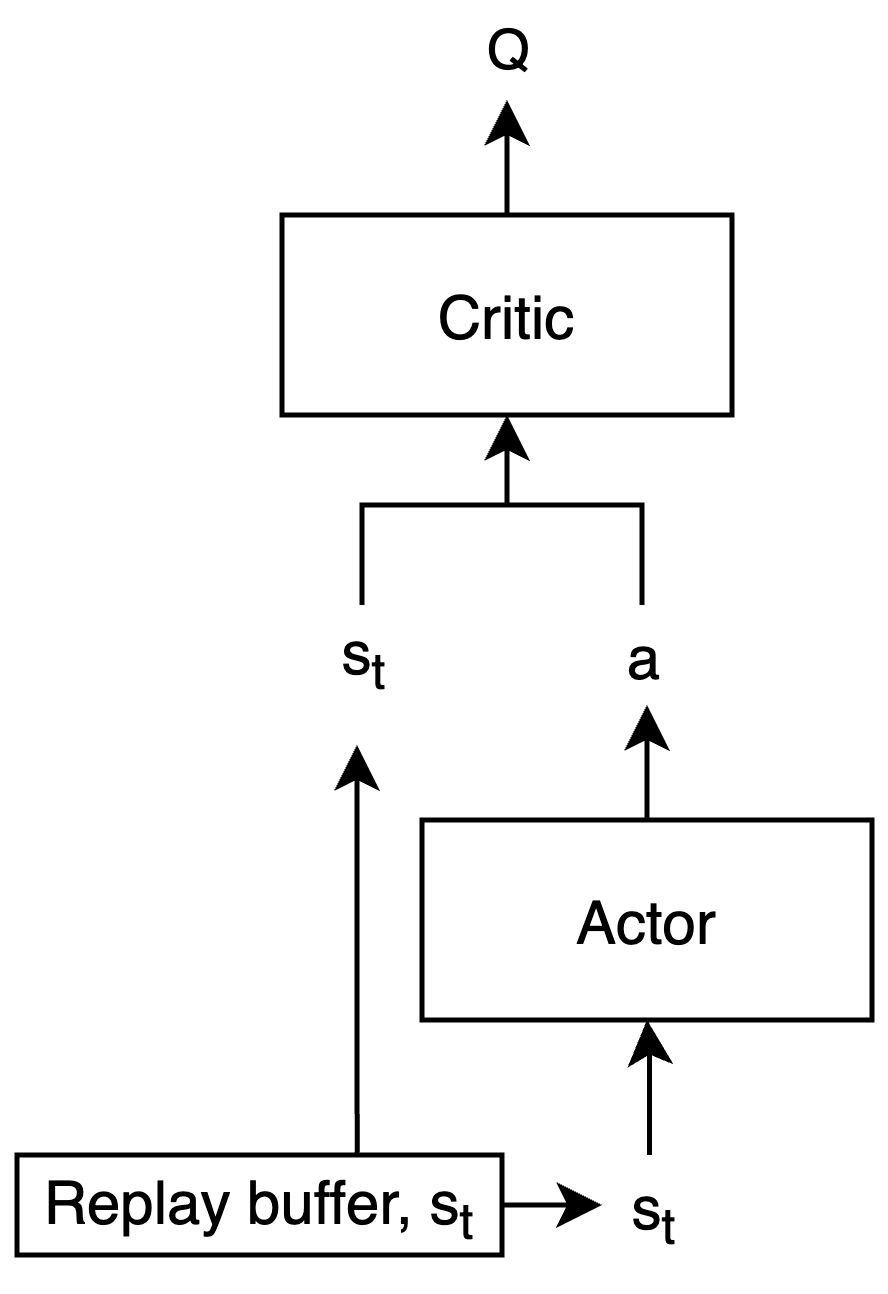
\includegraphics[width=\textwidth]{figures/3_/3_4_training_actor.png}
        \caption{Training the actor network}
        \label{fig:3_4_actor}
    \end{subfigure}
    \hfill
    \begin{subfigure}[b]{0.6\textwidth}
        \centering
        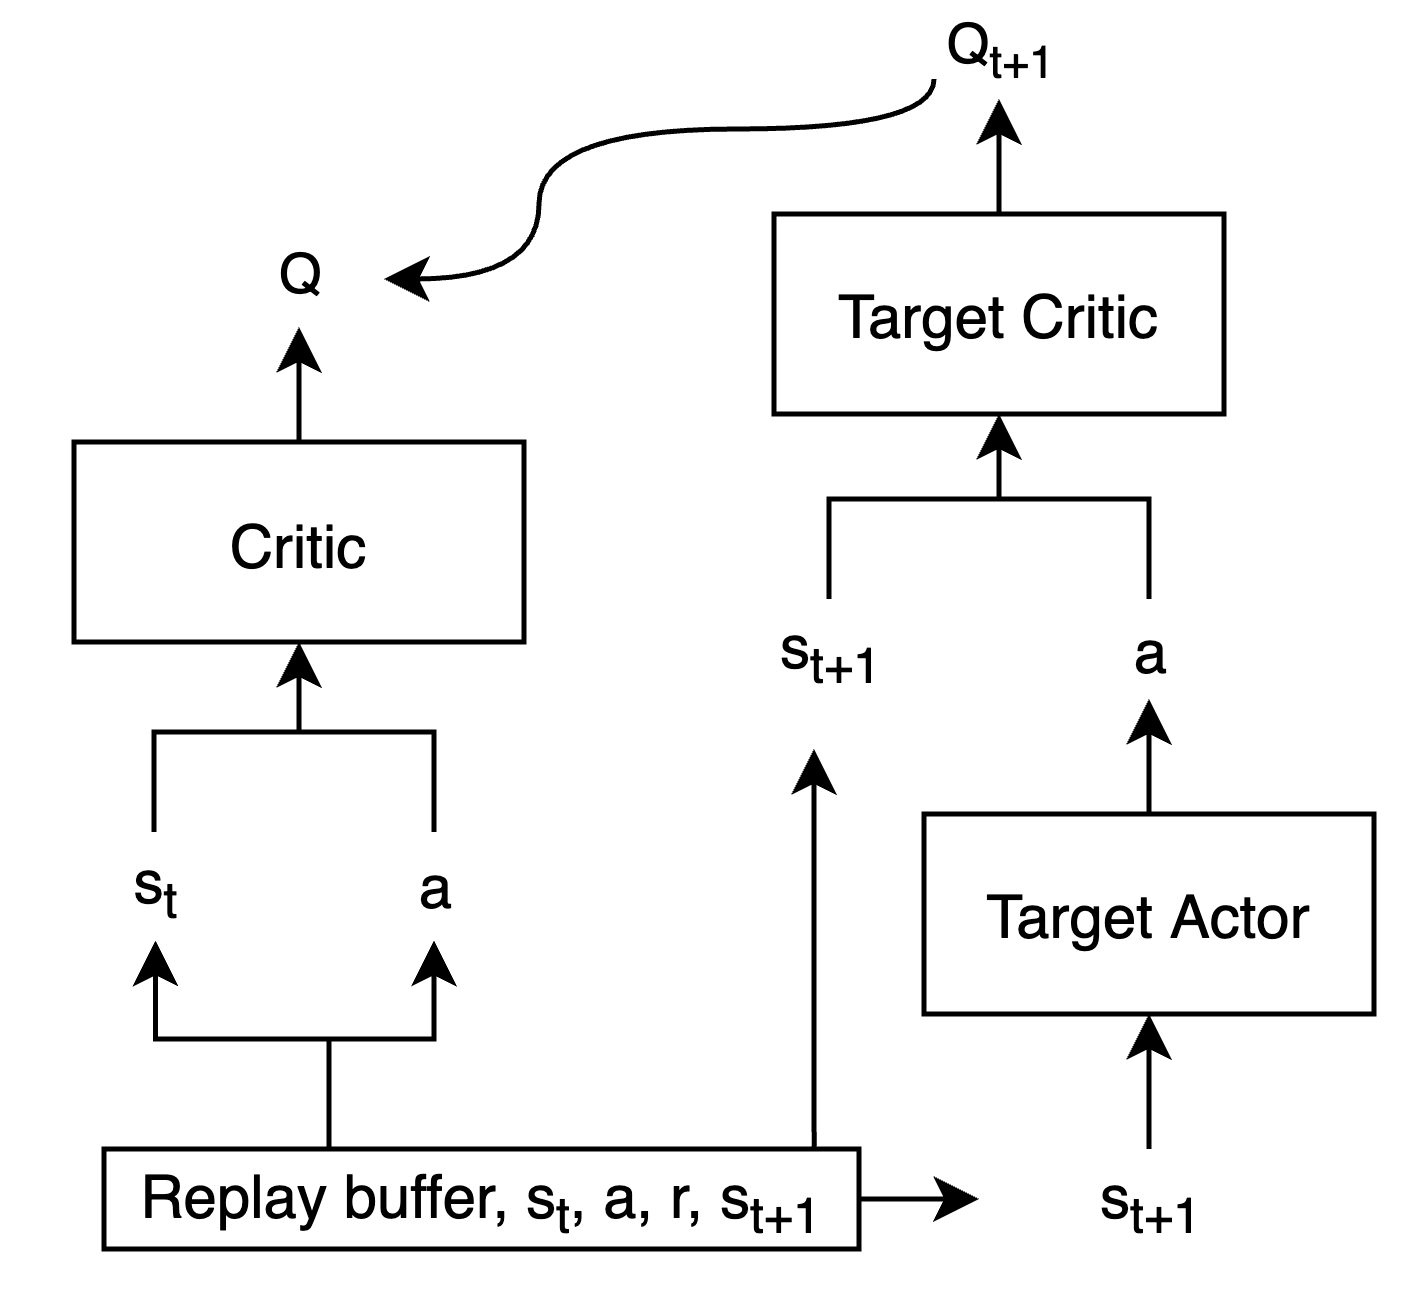
\includegraphics[width=\textwidth]{figures/3_/3_4_training_critic.png}
        \caption{Training the critic network}
        \label{fig:3_4_critic}
    \end{subfigure}
    \hfill
    \caption{An overview of how the actor and critic networks are updated in DDPG.}
    \label{fig:3_4_training}
\end{figure}
With a bit of understanding of the theory behind DDPG, it is insightful to have a more conceptual view over how DDPG is structured. From Figure \ref{fig:3_4_training}, we see that the actor network is updated as \eqref{3_4_actorGrad}, where the actor objective function $J(\btQ)$, which is $Q\,(S_t,\, \mu(S_t|\btmu)\,|\, \btQ)$, is backpropagated through the critic network and to the weights of the actor network. Similarly, we see that to obtain the prediction and the target of the loss in \eqref{3_4_NewcriticLoss}, we  sample the experience from the replay buffer, get our prediction term though our critic network, and get our target term through the target networks. Hence, we can calculate the MSE loss and backpropagate it to the critic network weights. Formally, backpropagation here simply refers to the method of calculating the gradient of the objective function or loss, with respect to the individual parameter weights of the network. Though informally, ``backpropagate it'' means to first find the gradient of the loss, w.r.t. the parameter weights, and then update the weights through gradient descent using the respective gradients.

\subsection{Summary}

DQN \cite{DQN} was able to solve Atari-based games from directly taking pixels as low-level observations as the state space. It was able to do this by adapting Q-learning \cite{watkins1992QLearning} with a NN as a parametrisation for the action-value function $Q$, along with the other innovations mentioned above. The universal function approximating ability of NNs allowed it to, in some sense, ``capture the features of the high dimensional observation space'', which allowed it to find an appropriate value estimate for each state with much fewer parameters than would otherwise be needed. So, by taking an image as input, the Q-network would have as output the value estimates for each possible action $a\in\mathcal{A}$ \cite{DQN}. The downside of this appears for problems that have high dimensional action spaces, as the size of output layer scales linearly with the number of actions.

DDPG follows the same idea as DQNs, but can in addition solve reinforcement learning problems with continuous (high-dimensional) observation and action spaces. 
This was achieved by using an actor-critic structure along with a NN parametrisation for the deterministic policy $\mu(s)$ and the action-value function $Q(s,a)$, where the additional actor gives DDPG the ability to learn how to output actions $a$, in the continuous action space, $\mathcal{A}$. Likewise, the critic $\Qt$, is able to take in this action $a$ along with an observation $s$, where both belong to continuous spaces, to output an appropriate action-value estimate. Then, to complete the cycle of the actor-critic structure, this action-value estimate can be used to train the actor network, as the gradient of the deterministic policy is simply the expected gradient of the action value function as shown in \eqref{3_4_actorGrad}. By being able to optimise this actor network to maximise its objective function, DDPG has thus the potential to obtain a policy capable of finding optimal actions in every state. 

Lastly, since DDPG is a model-free algorithm, it has the ability to perform well across learning tasks as it does not require any domain knowledge or transition dynamics, which follows from using \textit{Q}-learning to update the critic, as explained in Section \ref{sec:2_6_modelFreeContinuous}. This was also complemented by the fact that the DDPG uses \textit{batch normalisation}, so to generalise inputs into the actor and critic.
So with these characteristics, DDPG seems like a natural choice to use for the guidance task of this project.


\section{Proximal Policy Optimisation}
\label{sec:PPO}

In light of the advancements within reinforcement learning for robotics, a new family of methods was developed to curb the problem of instability and divergence when training agents using NNs. These are called \textit{trust-region} based policy optimisation methods, stemming from TRPO \cite{TRPO}.
PPO \cite{PPO} is heavily inspired by this, where the overarching idea is that in order to maintain stability in training, the new, updated policy should be within a specific \textit{trust-region} of the old policy, hence the name proximal policy.
As for its other characteristics, PPO is a also a model-free, on-policy and actor-critic method. In addition, it parametrises a stochastic policy $\pi(a\,|\,s)$ (unlike DDPG) and uses a uniquely defined objective function to optimise this.

\subsection{Advantage and some notation}
Earlier, we defined the policy gradient in \eqref{3_3_actorGrad}. This can be implemented in practice as:
\begin{equation}
    \widehat{\nbt J_t(\bt)} = \hatE \left[ 
    \frac{\nbt \pibt}{\pibt} \: \hatA (s, a) 
    \right] \label{3_5_actorGrad}
\end{equation}
where $\hatE$ represents the empirical average over a finite batch of samples of actions $a$ and states $s$. Also, we introduce a colloquial term $\hat{A}$, called the \textit{advantage} function $A : \mathcal{S} \times \mathcal{A} \rightarrow \mathbb{R}$, that represents how well an action did compared to some \textit{baseline} estimate:
\begin{equation}
    \hat{A}\,(s ,a) = \underbrace{Q\, (\,s,\, a\,)}_{\text{discounted return}} - \quad \underbrace{V_{\bt}\,(\,s\,)}_{\text{estimate}} \label{3_5_advantage}
\end{equation}
The baseline in this case is the parametrised value function $V_{\bt}$. Note that the first term shows the rewards that was actually received, while the second is an estimate of what we expected to receive in that state -- the critic. Hence, the advantage gives a picture of whether the agent performed better or worse than expected. 

We also introduce a slightly different notation here, where the subscript denotes the parameters to which the functions are parametrised with. Strictly speaking, the value functions should be taking in the random variables $S_t$ and $A_t$, but we assume the shorthand notation of $V_{\bt} (s) = V_{\bt} (S_t \,|\, S_t = s)$ for simplicity. This is also meant to prevent confusion with the advantage term $\hat{A}\,(s,a)$.

\subsection{PPO-Clip}
\label{subsec:PPO-clip}

PPO ensures that the new policy is close to the old one by using one of two tricks: clipping or an adaptive Kullback-Leibler (KL) divergence penalty term. Primarily, the one that is used is the \textit{clipped surrogate objective} version of PPO, which is also used in this project. In this version, the authors prevent large charges to the policy parametrisation by basically flattening the policy objective function to a certain maximum value. To visualise this, we can look at the novel objective function used.

PPO takes the surrogate objective function used by TRPO (whose gradient is equivalent to \eqref{3_5_actorGrad}):
\begin{equation}
    J_t(\bt) = \hatE \left[ 
    \frac{\pibt}{\pibtold} \: \hatA (s, a) 
    \right]
    = \hatE \left[ 
    r_t(\bt) \: \hatA (s, a) 
    \right]
\end{equation}
and clips it by a maximum value bounded by a hyperparameter $\epsilon$ to obtain the \textit{actor objective function}:
\begin{equation}
    J_t^{CLIP}(\bt) = \hatE \left[ \min\,(
    r_t(\bt) \: \hatA (s, a), \, \text{clip}\, ( r_t(\bt), 1-\epsilon, 1+\epsilon) \, \hatA(s,a)
    \right]
    \label{3_5_clippedObjective}
\end{equation}
This clipping aims to remove the incentive from deviating more than $\epsilon$ away from the old policy \cite{PPO} and can be visualised in Figure \ref{fig:3_5_clippedLoss}. Also, the ratio $r_t(\bt) = \frac{\pibt}{\pibtold}$ can be understood as the change in probability of selecting actions compared to the old policy, $\pibtold$, such that $r_t(\bt_{\text{old}}) = 1$.
\begin{figure}[htb]
    \centering
    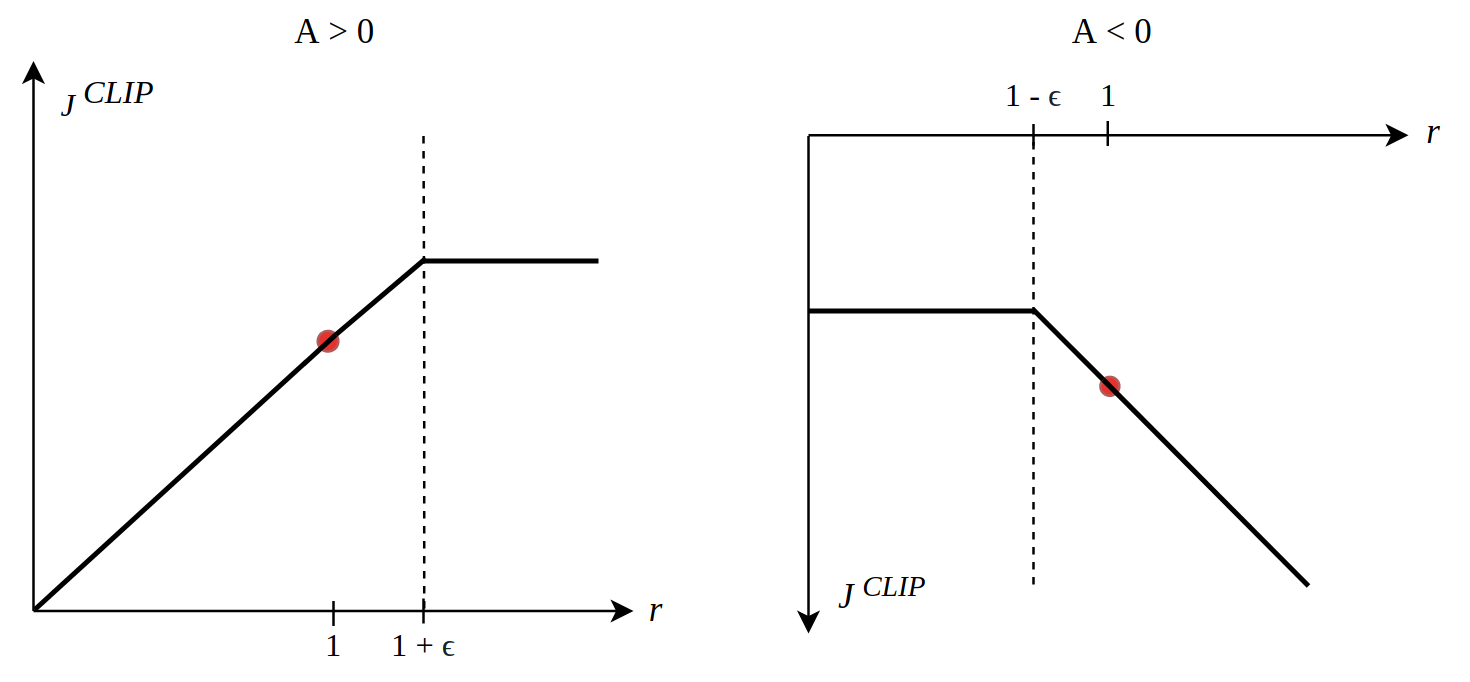
\includegraphics[width=0.8\textwidth]{figures/3_/3_5_clippedLoss.png}
    \caption{Visualising the clipped surrogate objective function for positive and negative advantages $A$. The figure is recreated from the original paper \cite{PPO}.}
    \label{fig:3_5_clippedLoss}
\end{figure}

The way to understand the clipped surrogate objective is to first remember that we are performing gradient ascent in the objective function, w.r.t. the policy parameters $\bt$. This means that we essentially choose the direction in which $r_t(\bt)$ should move in \eqref{3_5_clippedObjective} and Figure \ref{fig:3_5_clippedLoss}. When the agent performs better than expected, i.e. the advantage is positive, we wish to increase the probability of doing those actions again, which is equivalent to increasing $r_t(\bt)$. So, we adjust the parameters $\bt$ such that probability ratio $r_t(\bt)$ moves to the right. However, since we are taking the minimum and the objective is clipped at $1+\epsilon$, there is no added benefit of increasing $r_t(\bt)$ beyond this clipped point. Similarly, when the agent performs worse than expected, i.e. the advantage is negative, we wish to lower the probability of those actions happening again, which is equivalent to reducing the probability ratio $r_t(\bt)$. Again, since we clip the value at $1-\epsilon$ and the objective function is taking the minimum, there is no benefit of decreasing $r_t(\bt)$ beyond the clipped point. Therefore, by aiming to maximise the performance objective in \eqref{3_5_clippedObjective} by gradient ascent, the authors manage to prevent the new policy from deviating too far from the old one, as seen by $r_t(\bt)$ being discouraged to move beyond $[1-\epsilon, 1+\epsilon]$. 


\subsection{Actor-Critic Structure}
\label{subsec:3_ppo_actorCritic}
With the key idea from PPO presented, we can delve into the actor-critic structure of PPO. As shown above, the policy gradient is based on the advantage term $\hatA$. As a result, PPO uses a parametrisation of the value function $V(s)$ as a critic, so to produce an estimate for the advantage $\hatA$ in \eqref{3_5_advantage}.
Similarly to before \eqref{3_3_VE}, the parametrised value function can be optimised by minimising the mean-squared-error $\overline{VE}$:
\begin{equation}
    J_t^{VF}(\bt) = \E_t \Big[(V_{\bt_t}(s) - V_t^{\text{targ}})^2\Big] \label{3_5_criticLoss}
\end{equation}
where the target value function $V_t^{\text{targ}}$ that was implemented in the code of \cite{PPO} is defined as:
\begin{equation}
    V_t^{\text{targ}} = R_t + \gamma V_{\bt_t}(s')
\end{equation}
Lastly, there is an entropy term $S[\pi_{\bt}](s)$ that is also added to the objective function, which serves as an exploration term. 

So combined, the overall objective function for PPO with the actor objective function in \eqref{3_5_clippedObjective}, critic loss in \eqref{3_5_criticLoss} and entropy term, is:
\begin{equation}
    J_t^{CLIP+VF+S}(\bt) = \hatE \Big[
    J_t^{CLIP}(\bt) + c_1 J_t^{VF}(\bt) + c_2 S[\pi_{\bt}](s)
    \Big],   \label{3_5_objectiveFull}
\end{equation}
where $c_1$ and $c_2$ are coefficients. PPO also assumes that some automatic differentiation software is used, such that the software is able to keep track of how each objective function is computed in order to backpropagate the gradients appropriately. This also allows PPO to simply combine the objective functions like above.

Note that in the PPO implementation, the parameters $\bt$ characterise the whole actor-critic model, though ``under the hood'' they are indeed two different NNs that receive their own gradients. However, they have done this generalisation in the case where parameter-sharing is desired, where the ``bottom'' hidden layers are the same and the network heads are different. Moreover, since the actor is parametrising a stochastic policy, the head of the actor network outputs the parameters of the policy distribution, which for continuous cases is a Gaussian distribution.

Furthermore, one of the things to keep in mind is that PPO is also an on-policy algorithm. This means that when the agent is sampling experiences, these samples are gathered under its current policy $\pibt$. Hence, in its actor-critic implementation, a sample \textit{trajectory} of $T$ timesteps is first collected under a policy $\pibt$, before updates are made to the actor and critic parameters $\bt$. This means after $T$ timesteps, we have also received the rewards for each timestep and can compute the advantage estimates $\hatA$ for every timestep $t = 1, 2, ..., T$.
Then, when we are optimising the performance objective, we have the opportunity to define how many epochs $K$ was in that trajectory of size $T$, which means that we can specify how many gradient updates to do using the same batch of experiences. After the updates are completed, we discard this trajectory of experiences and begin sampling a new one, to ensure that the new experiences occur under the new policy $\pi_{\bt}$. 
\begin{figure}[ht]
    \centering
    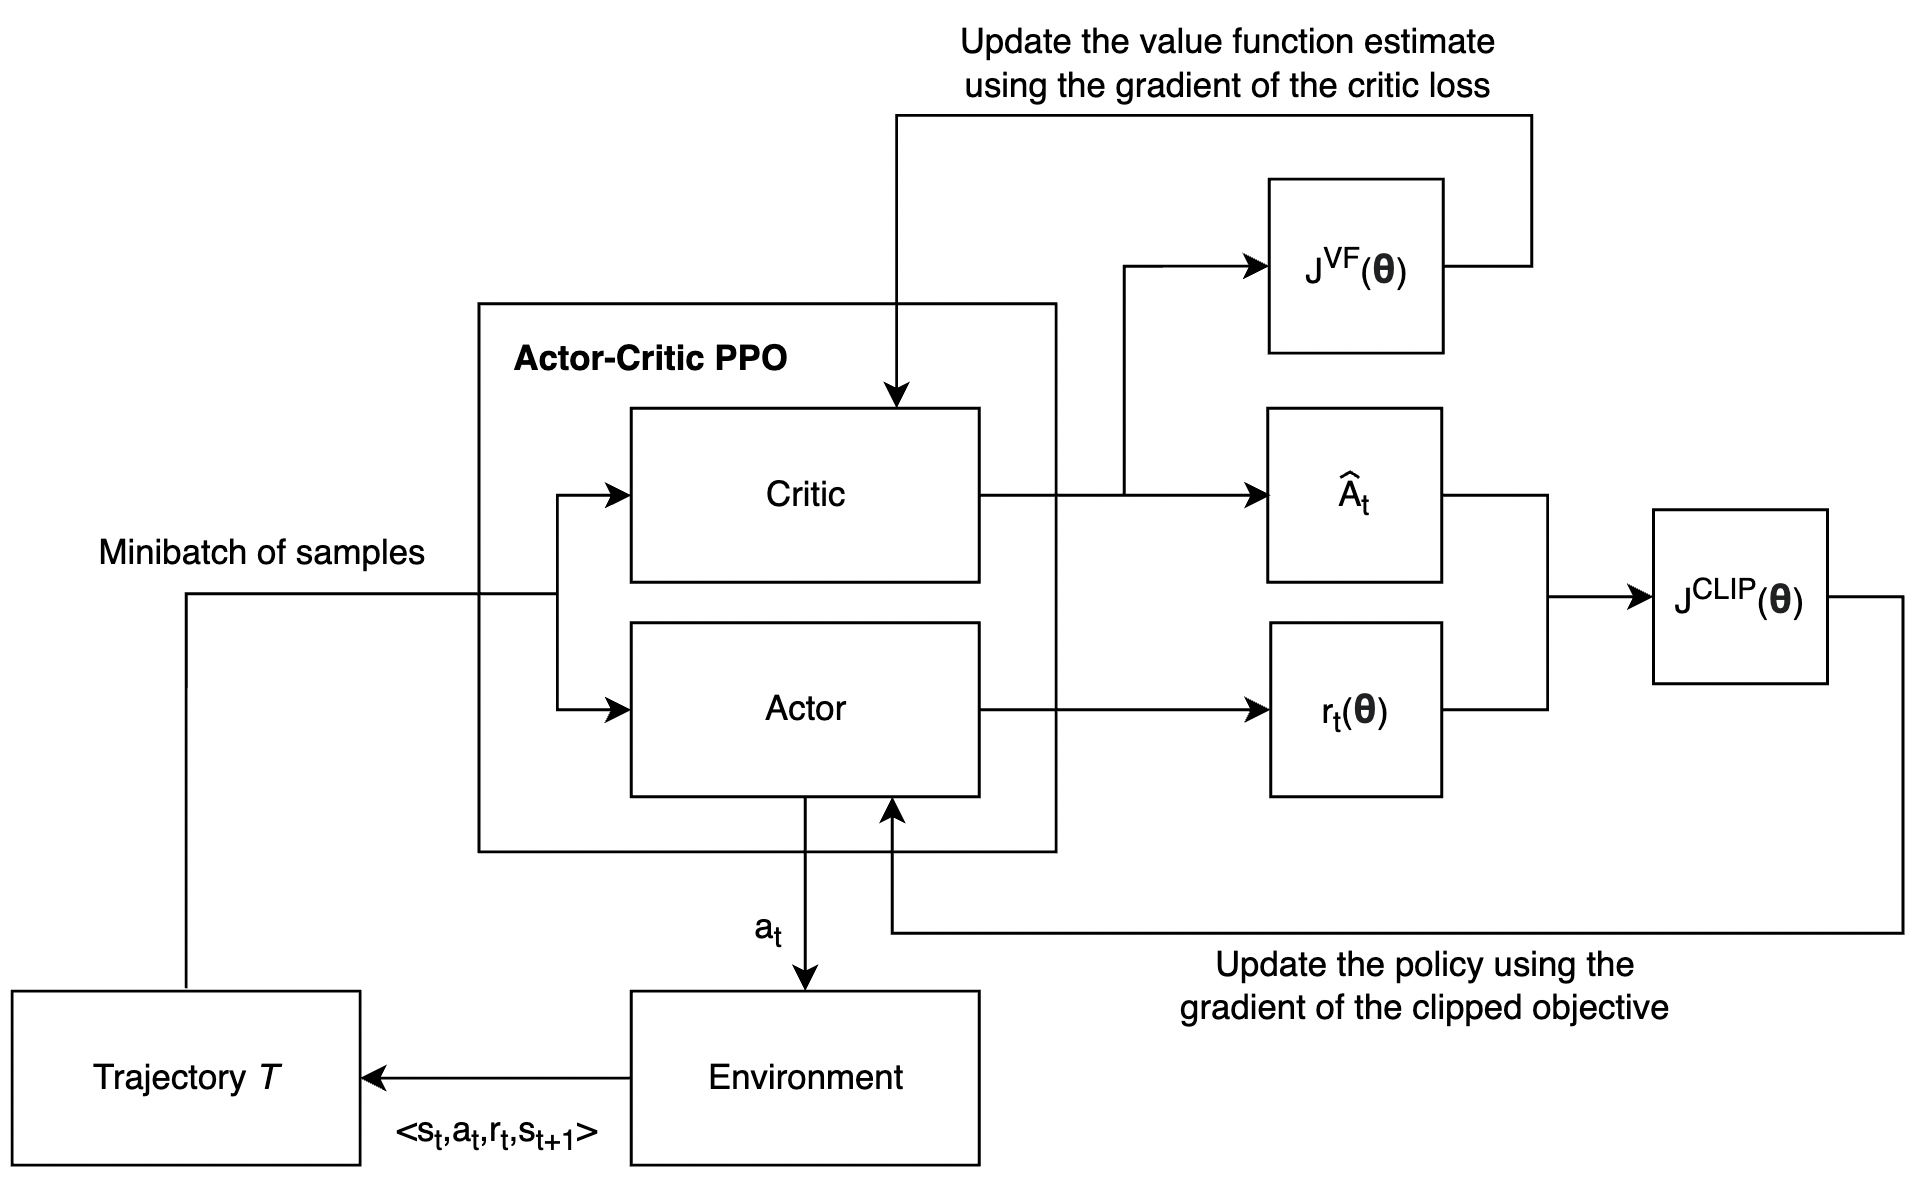
\includegraphics[width=0.95\textwidth]{figures/3_/3_5_ppoOverview.png}
    \caption{An overview of how the actor and critic networks are updated in PPO. Once the loss terms are calculated, the gradients $\nabla J_t^{CLIP}(\bt)$ and  $\nabla J_t^{VF}(\bt)$ are used to update the actor and critic respectively.}
    \label{fig:3_5_ppoTraining}
\end{figure}
Conceptually, we can view the whole update process in Figure \ref{fig:3_5_ppoTraining}. Here, we first see that a trajectory is sampled based on the current policy given by the actor, before the loss terms are calculated. Finally, the gradient of the objective function w.r.t. to the actor and critic weights is used to update the actor and critic networks.

\subsection{Summary}
PPO is able to solve a vast variety of continuous reinforcement learning problems by being a model-free, actor-critic method and using NNs as function approximators. It is also an on-policy method, meaning the sampled trajectory of experiences are collected under its current policy $\pibt$. The algorithm is able to achieve state-of-the-art performances through its adaptation of the trust-region based method, TRPO, where the idea is to take the largest possible step in the right direction, but while ensuring that the new policies, after an update, stay close (or are \textit{proximal}) to the old one. This in turn, as stated in TRPO \cite{TRPO}, should guarantee a monotonic improvement of the policy.

In terms of implementation, it is relatively simple compared to its counterpart, TRPO. It uses a clipped surrogate objective to define its proximal policy aim, rather than a hard constraint that requires second-order methods to optimise. Also, as it assumes we are using an automatic differentiation software, we can combine the objective functions for both the policy and the value function parametrisations, where the software is able to keep track of how to compute the gradients (perform backpropagation) for the respective parameters.

Also, since it is on-policy like TRPO, it retains its supposedly high data-efficiency and reliable performance. This is particularly significant for problems with high-dimensional state and action spaces, since the agent can focus on exploring actions along its current policy instead of obtaining needless gradients from actions in states that are very uncommon. This is also a reason why it is more data-efficient, as it is able to converge to an optimal behaviour faster.

However, since PPO is on-policy, the overall degree of exploration is based largely on its stochastic policy $\pibt$, with the exception of the entropy term. However, as discussed in the end of section \ref{sec:3_3_actor-critic}, this means that the agent may suffer from a lack of exploration if its policy does not incorporate some degree of randomness. Yet, by the nature of optimisation, PPO will progressively increase probabilities of doing ``good'' actions and decrease probabilities of doing ``bad'' ones, based on its estimate of advantage and value function. This means that over time, the agent will exploit the environment more, irrespective of how accurate its estimate of the policy and value function is, and could become trapped in a local optima.
